\documentclass[addpoints]{exam}

\usepackage{amsmath}
\usepackage{amssymb}
\usepackage{array}
\usepackage{geometry}
\usepackage{venndiagram}
\usepackage{graphicx}
\usepackage{tikz}
\usepackage{listings}
\usepackage{xcolor}
\usepackage{tabularx}
\usepackage{multicol}
\usepackage{multirow}
\usepackage{colortbl}
\usepackage{float}
% \usepackage{tcolorbox}
\lstset { %
    language=C++,
    backgroundcolor=\color{black!5}, % set backgroundcolor
    basicstyle=\footnotesize,% basic font setting
}

% Header and footer.
\pagestyle{headandfoot}
\runningheadrule
\runningfootrule
\runningheader{Computer Architecture}{Homework 3}{CE/CS - 321/330}
\runningfooter{}{Page \thepage\ of \numpages}{}
\firstpageheader{}{}{}

% \boxedpoints
\printanswers
\qformat{} %Comment this to number questions, uncomment this to not number questions

\newcommand\union\cup
\newcommand\inter\cap

\title{Computer Architecture}
\author{Ali Muhammad aa07190 | Section L3 \\ Iqra Ahmed ia07674 | Section L7} 
\date{Homework 3}
\begin{document}
\maketitle

\begin{center}
    \gradetable[h][questions]
\end{center}
\begin{sloppypar}
% \newpage
\begin{questions}
    \question[5]
    \begin{center} \textbf{Question 1: Pipeline Register Design [5 marks]} \end{center}

    What are the total number of bits needed for each pipeline register in the following pipelined RISC-V processor. Also break it down into the individual fields of each pipeline register and how many bits are needed for each field.

    \begin{figure}[ht]
        \centering
        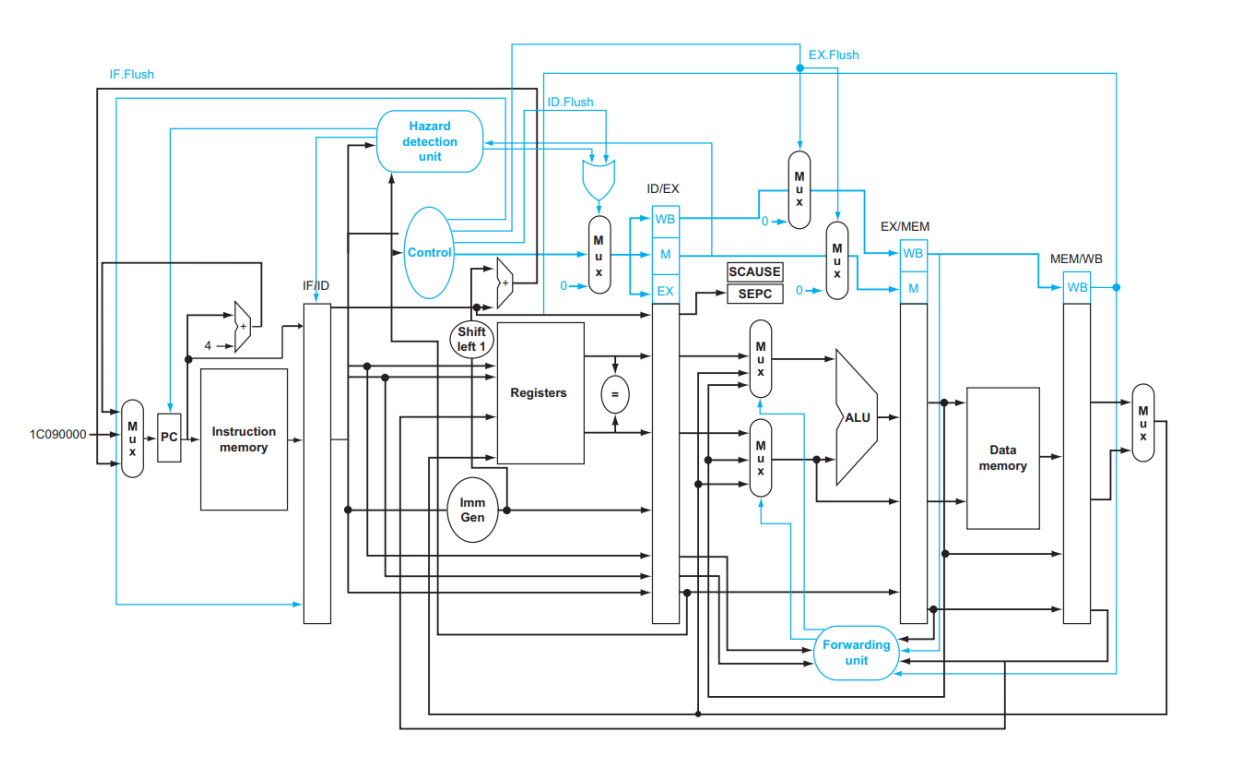
\includegraphics[scale = 0.5]{q1_fig.png}
    \end{figure}
    \begin{solution}
        
        The RISC-V Processor can be broken down into the following pipelines:
        \begin{enumerate}
            \item \textbf{\underline{IF / ID - Instruction Fetch / Instruction Decode:}} Program Counter (64 bits) and Instruction Memory that gives 32 bit instruction. \\ Total bits = 64 + 32= 96 bits.
            
            \item \textbf{\underline{ID / EX - Instruction Decode / Execute}} 
            
            Program Counter - 64 bits. \\ From Register File: ReadData1 (64 bits), ReadData2 (64 bits), RS1 (5 bits), RS2 (5 bits), RD (5 bits). \\ Immediate Generator - 64 bits. \\ ALUOp 4 bits, ALUSrc 1 bit \\ Branch, MemRead, MemWrite, MemtoReg, RegWrite each of 1 bit (5 bits in total) \\ 
            Total bits = 64 + 64 + 64 + 5 + 5 + 5 + 64 + 4 + 1 + 5 = 281 bits.

            \item \textbf{\underline{EX / MEM - Execute / Access operand from Data Memory:}}
            
            ALU Result - 64 bit. \\ Mux Out (ReadData2 or Immediate Value) - 64 bit. \\ RD - 5 bits. \\ 
            Left Shifted Immediate Value - 64 bit \\
            Branch, MemRead, MemWrite, RegWrite, MemtoReg each of 1 bit (5 bits in total) \\ Total bits = 64 + 64 + 64 + 5 + 5 = 202 bits.

            \item \textbf{\underline{Mem / WB - Memory / Write Back:}}
            
            Read\_Data from Data Memory - 64 bits. \\ 
            ALU Result - 64 bits. \\ RD - 5 bits \\ MemtoReg and RegWrite each of 1 bit (2 bits in total) \\ 
            Total bits = 64 + 64 + 5 + 2 = 135 bits.

            Total number of bits for each pipeline register in RISC-V pipelined processor = 96 + 281 + 202 + 135 = 714 bits.

            [The image given above is very vague without proper labeling, hence influence was taken from the pipelined RISC-V processor diagram given with the project details file.]
        \end{enumerate}
    \end{solution}
    \newpage
    \question[5]
    \begin{center}
        \textbf{Question 2: Pipeline Basics [5 marks]}    
    \end{center}

    In this exercise we examine how pipelining affects  the clock cycle time of the processor. Problems in this exercise assume that individual stages of the datapath have the following latencies: 

    \begin{tabular}{| l | l | l | l | l |}
            \hline
            IF \hspace*{17.5mm} & ID \hspace*{17.5mm} & EX \hspace*{17.5mm} & MEM \hspace*{17.5mm} & WB \hspace*{17.5mm} \\ \hline
            200ps & 300ps & 150ps & 350ps & 250ps \\ \hline
    \end{tabular}
    
    Also, assume that instructions executed by the processor are broken down as follows: 
    
    \begin{tabular}{| l | l | l | l |}
        \hline
        R-Type \hspace*{24.25mm}& beq \hspace*{24.25mm} & ld \hspace*{24.25mm} & sd \hspace*{24.25mm} \\ \hline
        40\% & 15\% & 20\% & 25\% \\ \hline
    \end{tabular}
    
    \begin{parts}
        \renewcommand{\thepartno}{\roman{partno}}
        \part What is the clock cycle time in a pipelined and non-pipelined processor? 
        \begin{solution}
            In pipelining, all stages must adhere to a single clock cycle that should be enough to accomodate the operation that takes the longest time. Therefore, for \underline{pipelined processor}, clock cycle time should be 350ps. \\ In non pipelining, each instruction would go through all stages and then new instruction would be executed. This happens in a single clock cycle, therefore, for a \underline{non-pipelined processor} clock cycle time = 200 + 300 + 150 + 350 + 250 = 1250ps. 
        \end{solution}
        \part What is the total latency of an ld instruction in a pipelined and non-pipelined processor?
        \begin{solution}
            An ld instruction takes all individual stages of a processor. 

            \underline{Pipelined:} Each stage would take 350ps since that is the clock cycle time. Total Latency = 350 * 5 = 1750ps.

            \underline{Non-Pipelined:} Each stage would take its own time. Total Latency = 200 + 300 + 150 + 350 + 250 = 1250ps.
        \end{solution}
        \part If we can split one stage of the pipelined datapath into two new stages, each with half the latency of the original stage, which stage would you split and what is the new clock cycle time of the
        processor?
        \begin{solution}
            Since the clock cycle time is based on the stage with the highest latency, it would be ideal to split the stage that takes the longest time. In our case that would be the MEM stage. \\ The new clock cycle time would then be the stage with the highest latency; ID - Instruction Decode with 300ps.
        \end{solution}
        \part Assuming there are no stalls or hazards, what is the utilization of the data memory?
        \begin{solution}
            Data Memory is only used by either ld, or sd instruction that take upto 20\% and 25\% of the processor. So utilization of the data memory is 20\% + 25\% = 45\% of the clock cycles.
        \end{solution}
        \part Assuming there are no stalls or hazards, what is the utilization of the write-register port of the ``Registers'' unit?
        \begin{solution}
            The write register is used by either R-Type instructions that require arithmetic operations or ld instruction as they require the data to be written. So utilization of write register = 40\% + 20\% = 60\% of the clock cycle time.
        \end{solution}
    \end{parts}

    \question[5]\begin{center}
        \textbf{Question 3: Pipeline Hazard Basics [5 marks]}
    \end{center}

    A hypothetical processor has 9 stages of a pipeline as shown in table below. The first row in the table below shows the pipeline stage number, second row gives the name of each stage, and third row gives the delay of each stage in Nano-seconds. The name of each stage describes the task performed by it. Each stage takes 1 cycle to execute. This processor stores all the register contents in a compressed fashion. After fetching the operands the operands are first decompressed, and before saving the results in register file, the results are first compressed.

    \begin{figure}[ht]
        \centering
        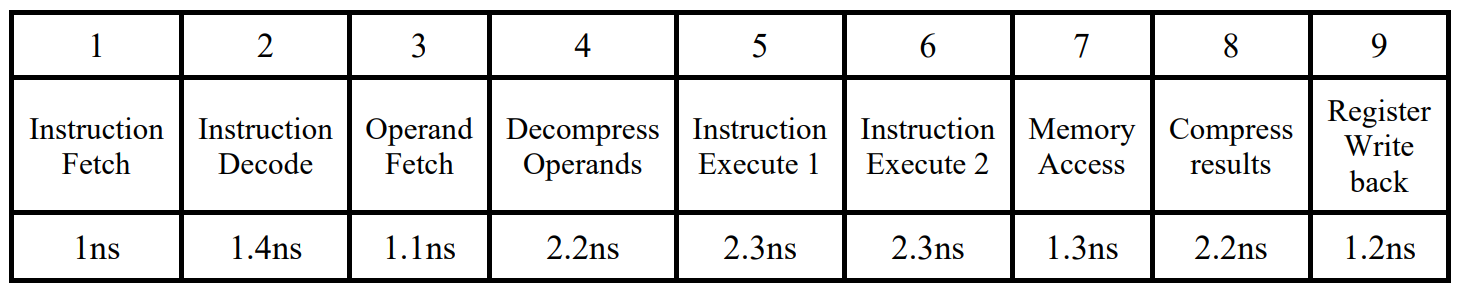
\includegraphics[scale = 0.45]{q3_fig.png}
    \end{figure}

    \begin{parts}
        \renewcommand{\thepartno}{\roman{partno}}
        \part How many cycles are required to implement/execute one instruction on this pipeline?
        \begin{solution}
            Since this is a 9 stage pipelined design, it'll take 9 clock cycles.
        \end{solution}
        \part How many cycles are required to execute 17 instructions on this pipeline? Assume that no stall cycles occur during the execution of all instructions.
        \begin{solution}
            17 instructions would take 17 cycles, plus the remaining stages left for the last cycle [overlaps hence can be considered like this.] \\ Total cycles = 17 + (9 - 1) = 25 cycles.
        \end{solution}
        \pagebreak
        \part Assume that all necessary bypass circuitry is implemented in this 9 stage pipeline. How many cycles will the pipeline stall during the execution of below given two instructions? \\ 
        \hspace*{10mm} \textrm{a. x5 = Load from memory} \\ 
        \hspace*{10mm} \textrm{b. x2 = x5 + x7} 
        \begin{solution}
            There will be 2 stalls assuming that all necessary bypass circuitry is implemented as when the instruction is loaded from memory in the Memory Access Stage, then it can be bypassed/forwarded to the Instruction Execute 1 stage which results in only \textbf{2 stalls}.
        \end{solution}
        \part Assume that no bypass circuitry is implemented in this 9 stage pipeline. How many cycles will the pipeline stall during the execution of above mentioned two instructions?
        \begin{solution}
            It will have an additional 2 stalls, as there is no bypass, then we have to wait for register write back, after which operand is fetched and decompressed before execution. So \textbf{4 stalls}.
        \end{solution}
        \part Assume that all necessary bypass circuitry implemented in this 9 stage pipeline. How many cycles will the pipeline stall during the execution of below given two instructions? \\ 
        \hspace*{10mm} \textrm{a. x5 = x1 + x3} \\ 
        \hspace*{10mm} \textrm{b. x2 = x5 + x7}
        \begin{solution}
            There should be 2 stalls again by similar logic as part (iii).
        \end{solution}
        \part Assume that no bypass circuitry is implemented in this 9 stage pipeline. How many cycles will the pipeline stall during the execution of above mentioned two instructions?
        \begin{solution}
            4 stalls by similar logic as part (iv).
        \end{solution}
        \part How much total time (in ns) is required to execute one entire instruction if the nine stages were \textbf{\underline{not pipelined}}?
        \begin{solution}
            Total time = 1 + 1.4 + 1.1 + 2.2 + 2.3 + 2.3 + 1.3 + 2.2 + 1.2 = 15.0ns
        \end{solution}
        \part What is the delay of 1 cycle (in ns) when all the nine stages are pipelined?
        \begin{solution}
            Delay should be of the instruction with highest latency; 2.3ns
        \end{solution}
        \part What is the total time (in ns) required to execute one entire instruction if the nine stages are pipelined?
        \begin{solution}
            Total time = time for 1 cycle $\times$ stages = 2.3 $\times$ 9 = 20.7ns
        \end{solution}
        \pagebreak
        \part Below are given two set of codes. For each set of code, mention if forwarding circuit can avoid all the stalls in the code? \\ 
        \hspace*{10mm} \textrm{a. \hspace*{3mm} add \hspace*{2mm} x1, x2, x3} \\ \hspace*{18.5mm} \textrm{add \hspace*{2mm} x6, x7, x8} \\ 
        \hspace*{18.5mm} \textrm{add \hspace*{2mm} x4, x1, x5} \\ 
        \hspace*{10mm} \textrm{b. \hspace*{3mm} ld \hspace*{4.5mm} x1, 0(x3)} \\ \hspace*{18.5mm} \textrm{add \hspace*{2mm} x2, x1, x3}
        \begin{solution}
            
            a. Stalls can be avoided by forwarding \\ 
            b. Stalls cannot be avoided by forwarding 
        \end{solution}
    \end{parts}
        
    \question[5]
    \begin{center}
        \textbf{Question 4: Pipeline Diagram [5 marks]}
    \end{center}

    Consider the following loop. \\
    \begin{tabular}{r l} 
        \texttt{LOOP:} & \texttt{ld x11, 8(x13)} \\ 
        & \texttt{ld x10, 0(x13)} \\ 
        & \texttt{add x12, x10, x11} \\ 
        & \texttt{addi x13, x13, -16} \\ 
        & \texttt{bne x12, x0, LOOP}
    \end{tabular}

    Assume that perfect branch prediction is used (no stalls due to control hazards), that the pipeline has full forwarding support, and that branches are resolved in the EX (as opposed to the ID) stage. 
    \begin{parts}
        \renewcommand{\thepartno}{\roman{partno}}
        \part Show a pipeline execution diagram for the first two iterations of this loop.
        \part Mark pipeline stages that do not perform useful work. How often while the pipeline is full do we have a cycle in which all five pipeline stages are doing useful work?
    \end{parts}
    \begin{EnvFullwidth}
        \begin{solution}
            (i) and (ii) [Zoom in to see a better picture, can be zoomed in.]
            \begin{figure}[H]
                \centering
                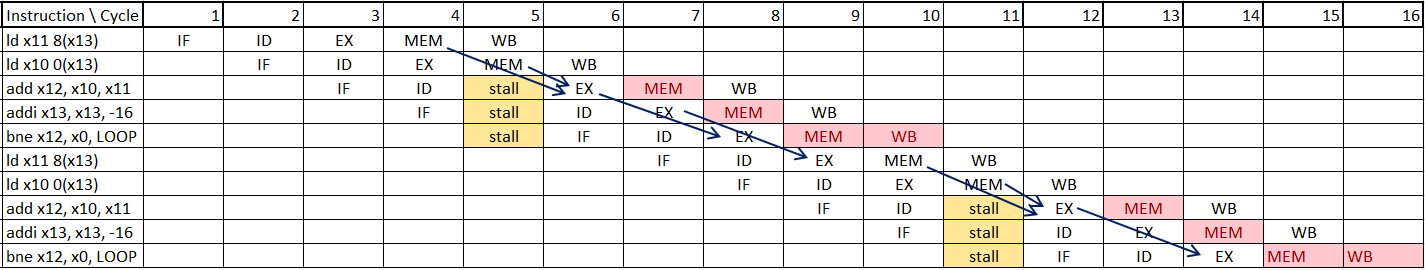
\includegraphics[scale = 0.4775]{q4_ans_i.png}
            \end{figure}
            The dark blue arrows show where forwarding has been done. The yellow boxes show where there is a stall and the red boxes show stages in the pipeline where no useful work is being performed. As it can be seen clearly that we do not have any cycle in the pipeline during which all five stages are performing useful work.
        \end{solution}    
    \end{EnvFullwidth}
    
    \question[5]
    \begin{center}
        \textbf{Question 5: Energy Consideration in Pipeline Design [5 marks]}
    \end{center}

    This exercise explores energy efficiency and its relationship with performance. Problems in this exercise assume the following energy consumption for activity in Instruction memory, Registers, and Data memory. You can assume that the other components of the datapath consume a negligible amount of energy. (“Register Read” and “Register Write” refer to the register file only.)

    \begin{tabular}{| l | l | l | l | l |}
        \hline
        I-Mem \hspace*{4.5mm}& 1 Register Read\hspace*{4.5mm} & Register Write\hspace*{4.5mm} & D-Mem Read\hspace*{4.5mm} & D-Mem Write\hspace*{4.5mm} \\ \hline
        120pJ & 80pJ & 60pJ & 120pJ & 100pJ \\ \hline 
    \end{tabular}

    Keep in mind that reading two registers (instead of one) will double the energy consumption of register reading. Assume that components in the datapath have the following latencies. You can assume that the other components of the datapath have negligible latencies.

    \begin{tabular}{| l | l | l | l | l |}
        \hline
        I-Mem\hspace*{5.75mm} & Control\hspace*{5.75mm} & RegisterReadorWrite\hspace*{5.75mm} & ALU \hspace*{5.75mm} & D-MemReadorWrite\hspace*{5.75mm} \\ \hline
        200ps & 150ps & 90ps & 90ps & 250ps \\ \hline
    \end{tabular}

    \begin{parts}
        \renewcommand{\thepartno}{\roman{partno}}
        \part How much energy is spent to execute an add instruction in a single-cycle design and in the five-stage pipelined design?
        \begin{solution}
            The energy spent will remain the same for a single add instruction in both the single-cycle and five-staged pipelined design. I-Mem, 2 register reads, and 1 register write. Energy = 120 + 2(80) + 60 = 340pJ.
        \end{solution}
        \part What is the worst-case RISC-V instruction in terms of energy consumption? What is the energy spent to execute it?
        \begin{solution}
            The worst instruction would be that takes the most energy in total. We either have two read registers at most, such as the add instruction, however, it does not utilise all the components. Now consider the load (ld) instruction that has a register read and a register write. Energy for ld = 120 + 2(80) + 60 + 120 = 460pJ. So the worst instruction would be the load instruction taking 460pJ of energy for execution.
        \end{solution}
        \part If energy reduction is paramount, how would you change the pipelined design? What is the percentage reduction in the energy spent by an ld instruction after this change?
        \begin{solution}
            I-Mem has to be done for all instructions, and so does Register Read. I-Mem can't be modified, however, we can modify the Register Read such that it takes 2 signals; RegRead1 and RegRead2. Then whatever signal will be activated by the contol unit (depending on the instruction), only that register will be read. This way, both registers will not have to be read for every instruction, such as the load instruction. We do not modify Register Write, D-Mem Read or D-Mem Write, as they are only performed when signal is active for those operations for those instructions.

            Now ld instruction takes energy = 120 + 80 + 60 + 120 = 380pJ. 

            Percentage reduction in energy = $ \displaystyle\frac{80}{460} \times 100 = 17.4\% $
        \end{solution}
        \part What other instructions can potentially benefit from the change discussed in (iii)?
        \begin{solution}
            All I-Type instructions would benefit from this such as \texttt{addi} as they only require one register read. \texttt{jal} instruction would also benefit as it does not read any registers.
        \end{solution}
        \part How do your changes from (iii) affect the performance of a pipelined CPU?
        \begin{solution}
            Previously, the Control Unit would decode the instructions while registers were being read simultaneously. Now the Control Unit would have to decode the instruction before in order to decide which registers to read. Hence, the Control Unit and Register Reads cannot be done at the same time, and would require seperate stages or clock cycles. This would increase the latency of the ID stage (Instruction Decode) as to accomodate the Control Unit as well and could potentially increase the clock cycle time of the processor [although in this question this is not the case, but it can be in some cases].
        \end{solution}
        \part We can eliminate the MemRead control signal and have the data memory be read in every cycle, i.e., we can permanently have MemRead=1. Explain why the processor still functions correctly after this change. If 25\% of instructions are loads, what is the effect of this change on clock frequency and energy consumption?
        \begin{solution}
            If MemRead control signal is always set to 1, then either it is needed by some instruction such as the load instruction, or it is not needed such as the add instruction in which case it is ignored in the MUX after the data memory as it is not needed and MUX does not select it, so is not written anywhere. So the processor still functions correctly. 
            
            If 25\% instructions are load, then remaining 75\% instructions are not load. There is no effect on the clock frequency, however, the energy consumption would most certainly increase due to the number of unnecessary Memory Reads on the remaining 75\% instructions. So increase in energy consumption would be of 120pJ in the remaining 75\% instructions of clock cycle time of 250ps. 
            Energy increase = $ \frac{120 \times 75\%}{250} = 0.36 $
        \end{solution}
    \end{parts}
\pagebreak
    \question[5]
    \begin{center}
        \textbf{Question 6: Pipeline Design Optimization for Memory Access [5 marks]}
    \end{center}

    ld is the instruction with the longest latency on the RISC-V implementation of single-cycle non-pipelined processor discussed in class. If we modified ld and sd so that there was no offset (i.e., the address to be loaded from/stored to must be calculated and placed in rs1 before calling ld/sd), then no instruction would use both the ALU and Data memory. This would allow us to reduce the clock cycle time. However, it would also increase the number of instructions, because many ld and sd instructions would need to be replaced with ld/add or sd/add combinations.

    \begin{parts}
        \renewcommand{\thepartno}{\roman{partno}}
        \part What would the new clock cycle time be for non-pipelined processor?
        \begin{solution}
            It would be the sum of the latencies of all individual stages of the processor; 600ps [from Dr. Soorat's slides.] 

            Since the question is vague, I took latencies from slides of Dr. Soorat which had 800ps total latency, and 200ps latency for the Execution stage. So without the Execution stage, the clock cycle time for non-pipelined processor would be 600ps.
        \end{solution}
        \part In the non-pipelined version, would a program with the instruction mix presented in Question 2 run faster or slower on this new CPU? By how much? (For simplicity, assume every ld and sd instruction is replaced with a sequence of two instruction.)
        \begin{solution}
            CPU Time$_{Before} = 200 + 300 +150 + 350 + 250 = 1250ps$ \\
            Load and Store instructions comprise of 45\% of instructions. \\  
            CPU Time$_{New} = 1.45 * (200 + 300 + 350 + 250) = 1.45 * 1100 = 1595ps $.

            Speedup = $ \displaystyle\frac{1250}{1595} = 0.784 $. 
            
            The new CPU will run 0.784 times slower.
        \end{solution}
        \part What is the primary factor that influences whether a program will run faster or slower on the new CPU?
        \begin{solution}
            The primary factor that influences the speed of a program are the number of load and store intructions. In addition, the way load and store instructions are made can also have an effect; if load and store have only few different addresses, then it may also run somewhat faster.
        \end{solution}
        \part Do you consider the original CPU a better overall design; or do you consider the new CPU a better overall design? Why?
        \begin{solution}
            I consider the original CPU a better overall design. Even though the old CPU design has a longer clock cycle, it still has much fewer instructions. Generally, load and store instrucitons are the primary factors that influence the speed of the program. If load and store are further broken down along with add instructions to calculate offset, this would increase the number of instructions and complexity of the design as now the offset would have to be calculated by the add instruction, and then stored later on for the load and store instructions to use, so more hardware components or signals would have to be used accordingly. This would undoubtedly increase the complexity of the processor. Moreover, the increase in number of instructions might also cause the processor to perform even slower.
        \end{solution}
        % \pagebreak
        \part As a result of the change, the MEM and EX stages of the pipelined version of the processor can be overlapped and the pipeline has only four stages. How will the reduction in pipeline depth affect the cycle time?
        \begin{solution}
            The reduction will only effect cycle time if the stage with the longest stage has been affected such that its cycle time is reduced. Since they are only overlapped and not changed in any way, the clock cycle time will not be changed as longest latency time would still remain same.
        \end{solution}
        \part How might this change improve the performance of the pipeline?
        \begin{solution}
            For lesser instructions with fewer load and store instructions, the new CPU would perform better.
        \end{solution}
        \part How might this change degrade the performeance of the pipeline?
        \begin{solution}
            For more number of instructions with higher number of load and store instructions, the new CPU would perform poorly as compared to the old CPU design.
        \end{solution}
    \end{parts}
    \pagebreak
    \question[50]
    \begin{center}
        \textbf{Question 7: Pipeline Design for New Instructions [50 marks]}
    \end{center}

    Consider the following instructions that are not found in the RISC-V architecture:

    \begin{tabular}{r  l  l }
        i. & \texttt{Load Word Register} &  \\
        &  \textrm{lwr rd, rs2(rs1)} & // Reg[rd] = Mem[Reg[rs1] + Reg[rs2]] \\ 
        ii. & \texttt{Add 3 Operands} & \\ 
        & \textrm{add3 rd, rs1, rs2, rs3} & // Reg[rd] = Reg[rs1] + Reg[rs2] + Reg[rs3] \\ 
        iii. & \texttt{Add to Memory} & \\ 
        & \textrm{addm rd, Offset(rs)} & // Reg[rd] = Reg[rd] + Mem[Offset + Reg[rs]] \\ 
        iv. & \texttt{Branch Equal to Memory} & \\ 
        & \textrm{beqm rs1, offset(rs2), rs3} & // if(Reg[rs1] == Mem[Offset + Reg[rs2]]) \\ 
        & & //\hspace*{10mm} PC = PC + Reg[rs3] \\ 
        v. & \texttt{Store Word and Increment} & \\ 
        & \textrm{swinc rs2, offset(rs1)} & // Mem[Reg[rs1] + offset] = Reg[rs2], \\ & & // Reg[rs1] = Reg[rs1] + 4 \\         
    \end{tabular}

    We want to modify the RISC-V processor to support the above instructions. For parts (b) and (d) below, you can use a printed version of the figures in the book over which you can draw your suggested modifications (no need to draw the entire diagram from scratch).

    For each of the above instructions, do the following: 
    \begin{parts}
        \part (1 mark) Suggest if any of the existing instruction formats is a good choice to encode the new instruction. If not, then propose a new instruction format. 
        \part (3 marks) Modify the datapath and control signals of the single-cycle RISC-V processor (Figure 4.17 of the book) to execute the new instruction using the instruction format suggested in part (a). Use the minimal amount of additional hardware and clock cycles/control states. Remember when adding new instructions, don't break the operation of the standard ones.
        \part (1 mark) Discuss the effect of the modification in part (b) on the latency of single-cycled non-pipelined CPU 
        \part (2 marks) Discuss if the suggested modification in part (b) should be handled by increasing/decreasing the number of pipelining stages that were discussed in class. Draw a pipelined version of the new processor similar to Figure 4.49 of the book. 
        \part (2 marks) Disucss if any new types of data hazards are introduced due to the new instruction? If yes, can they be mitigated through forwarding? Use a mutli-cycle pipeline diagram like Figure 4.51 of teh book to illustrate the new forwarding paths.
        \part (1 mark) Discuss, based on the above analysis, why the new instruction was not made part of the RISC-V architecture.
    \end{parts}
    \newpage
    \begin{solution}
        \begin{parts}
            \renewcommand{\thepartno}{\roman{partno}}
            \part \underline{\texttt{Load Word Register}} 

            \texttt{lwr rd, rs2(rs1)} \hspace*{5mm} // Reg[rd] = Mem[Reg[rs1] + Reg[rs2]]
            \begin{subparts}
                \renewcommand{\thesubpart}{\alph{subpart}}
                \subpart We can see that this lwr instruction is similar to the R-Type instruction. So we can use the existing R-Type instruction format along with some modification to implement the lwr instruction. The R-Type can be made as follows: 7-bit Opcode, 5-bit RD, 3-bit Funct3, 5-bit RS1, 5-bit RS2, 7-bit Funct7
                \subpart Since the instruction deals with memory read, and register write, the control signals of the traditional R-Type won't work, and would have to be modified:

                ALUSrc = 0 to add rs2 to rs1 for the offset, ALUOp = 10 (same as add), RegWrite = 1 for write back into RD, MemWrite = 0, MemRead = 1 as memory is read, and MemtoReg = 1 as data from Memory is written on register RD. 

                The datapath for \texttt{lwr} is as follows (red lines show active datapath - not including control signals for which values are written along with the signal):
                \begin{figure}[H]
                    \centering
                    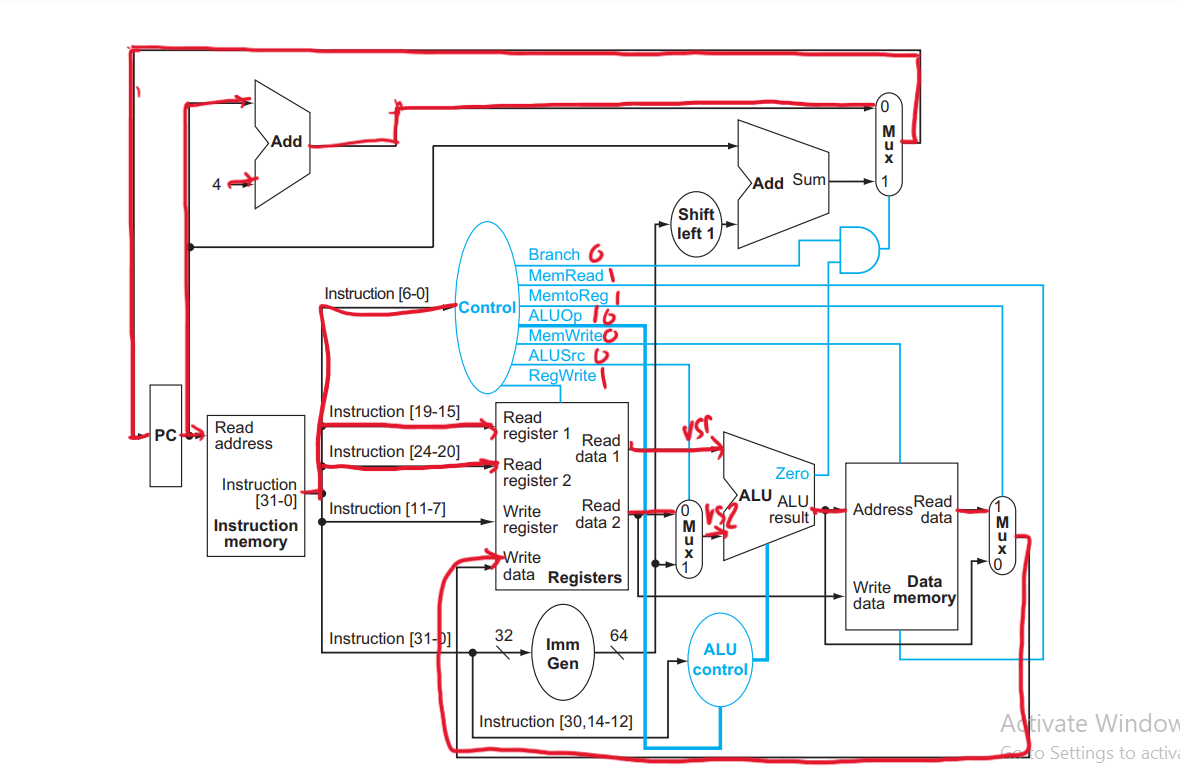
\includegraphics[scale = 0.5]{Q7_b_lwr.png}
                \end{figure}

                \subpart The latency of single-cycled non-pipelined CPU would remain the same.
                \pagebreak
                \subpart No changes are needed so the pipelined processor remains same as shown:
                \begin{figure}[H]
                    \centering
                    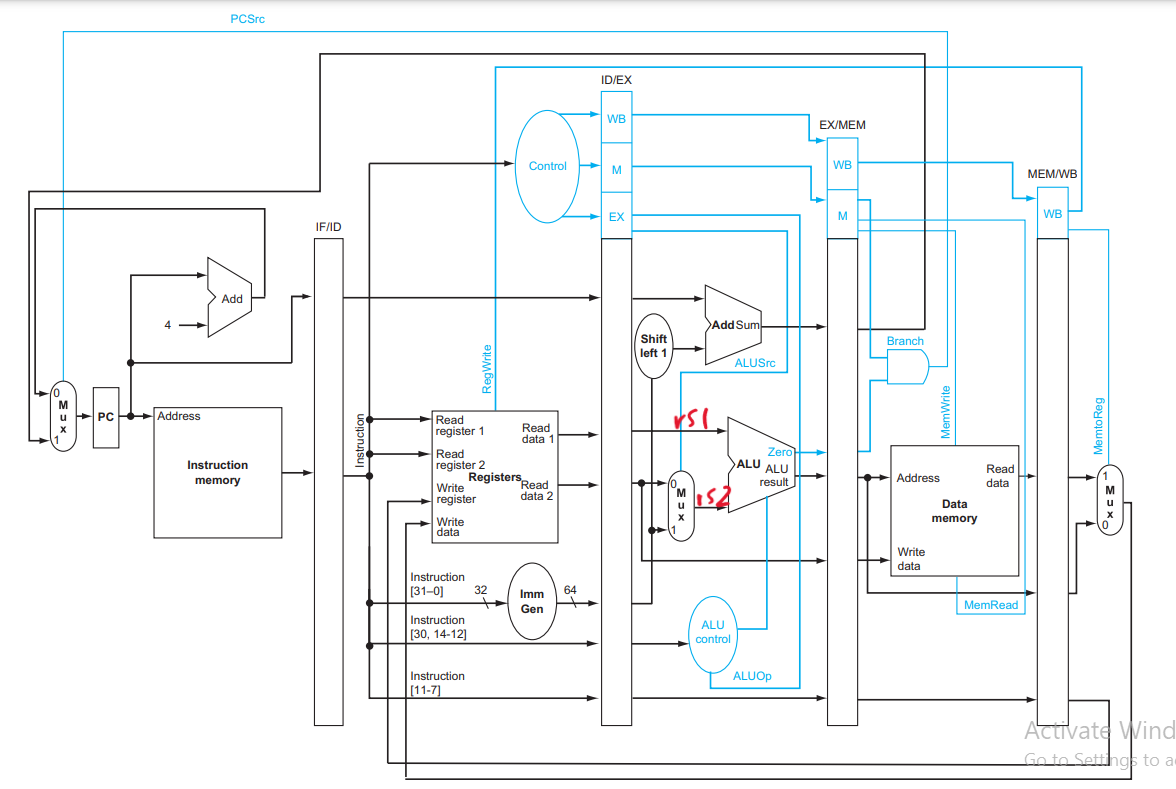
\includegraphics[scale = 0.55]{Q7_d_lwr.png}
                \end{figure}

                \subpart no new data hazards would be introduced.
                \subpart RISC-V architecture is the simplest architecture and supports the basic instructions, while lwr is a complex instruction. Hence was not made part of the RISC-V architecture. Also it does not make much sense to add register value as an offset when the \texttt{ld} instruction already exists which basically performs the same task.
            \end{subparts}
\newpage
            \part \underline{\texttt{Add 3 Operands:}} 
            
            \texttt{add3 rd, rs1, rs2, rs3} \hspace*{5mm} // Reg[rd] = Reg[rs1] + Reg[rs2] + Reg[rs3]
            \begin{subparts}
                \renewcommand{\thesubpart}{\alph{subpart}}
                \subpart Since there is no format that can deal with three operand instructions, we can define a new instruction format and label it as ``T-Type" where T denotes three operand instruction. The instruction can be divided as follows: 7-bit Opcode [custom opcode], 5-bit RD, 5-bit RS1, RS2, and RS3 each, and a 5-bit funct5 value [custom funct5 value].
                \subpart Since we are dealing with 3 operands, the register file would have to be modified to include an additional third register RS3 value, and a ReadData3 value that reads the value from the third register. The ALU would also have to be modified to include 3 operands which can be implemented with an additional MUX that can send the ReadData3 value - the new MUX would be controlled by another signal; ALUSrcB that indicates a third register value. We would need another ALUOp value for the ALU that indicates three operand instructions, and can support various operations between them - ALUOp would then become a 5 bit value. 

                The datapath for \texttt{add3} is as follows:
                \begin{figure}[H]
                    \centering
                    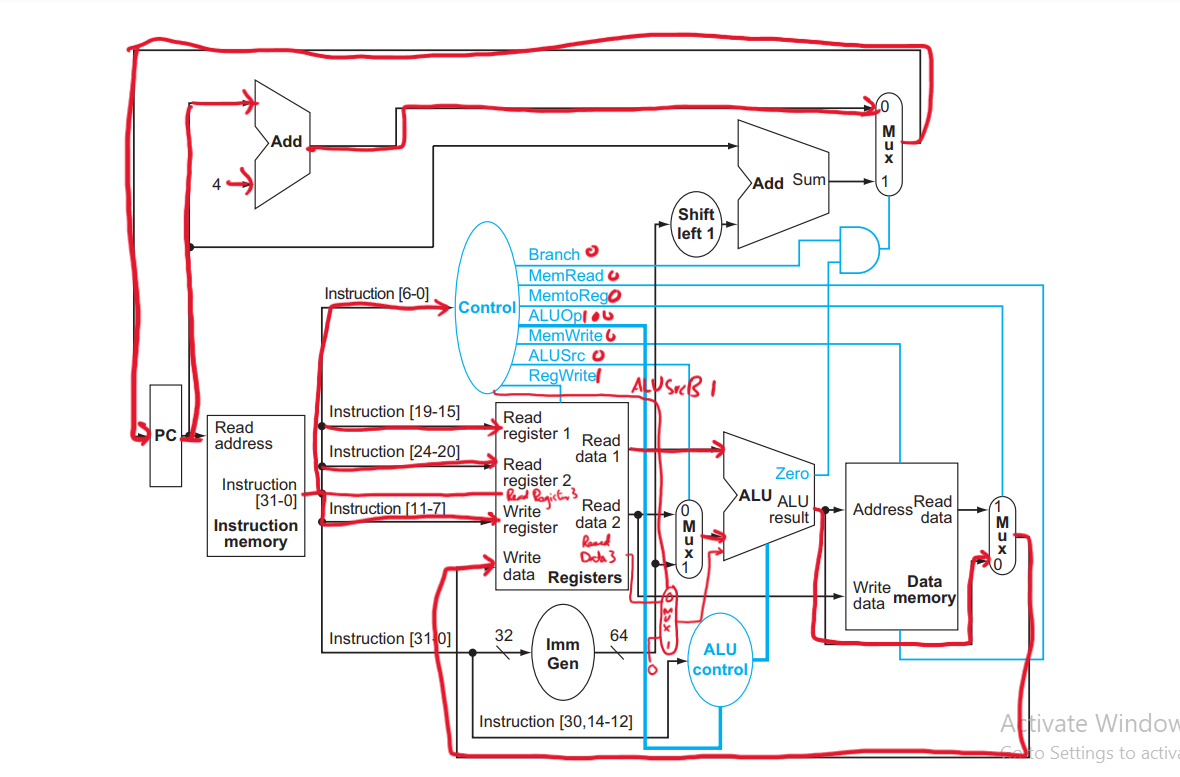
\includegraphics[scale = 0.5]{Q7_b_add3.png}                    
                \end{figure}

                \subpart It would definitely increase the latency, as now we would require three register reads, three register value outputs, and three ALU operands. So each of the ID stage, and EX stage would then take more time and hence increased latency.
                \subpart  It can be handled with the same number of pipeline stages, however, we would require an increased number of registers at some stages (ID/EX and EX/MEM) and would have to handle more signals as shown: 
                \begin{figure}[H]
                    \centering
                    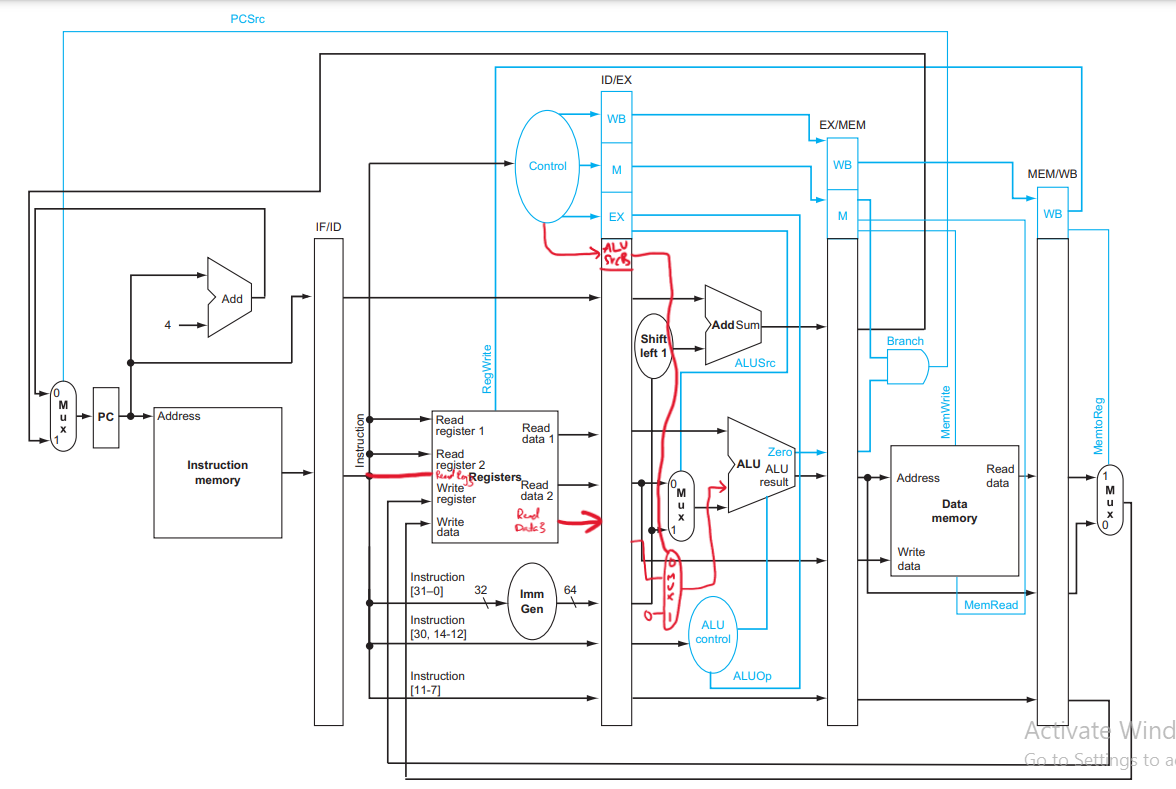
\includegraphics[scale = 0.5]{Q7_d_add3.png}                    
                \end{figure}

                \subpart There wouldn't be any new data hazard signals, only the previous ones such as a data hazard which can be mitigated through forwarding. 
                \subpart RISC-V architecture is the simplest architecture. Adding this instruction would increase the complexity, hence it was not added to the RISC-V architecture, as the same instruction can be performed by the use of two add instructions as well. 
            \end{subparts}
            \newpage
            \part \underline{\texttt{Add to Memory}}
            
            \texttt{addm rd, Offset(rs)} \hspace*{5mm} // Reg[rd] = Reg[rd] + Mem[Offset + Reg[rs]]
            \begin{subparts}
                \renewcommand{\thesubpart}{\alph{subpart}}
                \subpart This instruction deals with both a register operand, and memory access. However, it seems similar to the \texttt{ld} instruction format. So we can encode the \texttt{addm} instruction using the I-Type instruction format: 7-bit Opcode, 5-bit RD, 3-bit Funct3, 5-bit RS, 12-bit Immediate value.
                \subpart Since we are adding the value of the offset to RS, and then further adding it to RD, we can implement an additional MUX to the write back signal that chooses between an adder value of RD generated from the Register File, or the simple write back from memory - a signal ``Addm'' would be given from the control unit. If the signal is 1, then added value is selected, else the original write back value is selected. The datapath then becomes as shown: 
                \begin{figure}[H]
                    \centering
                    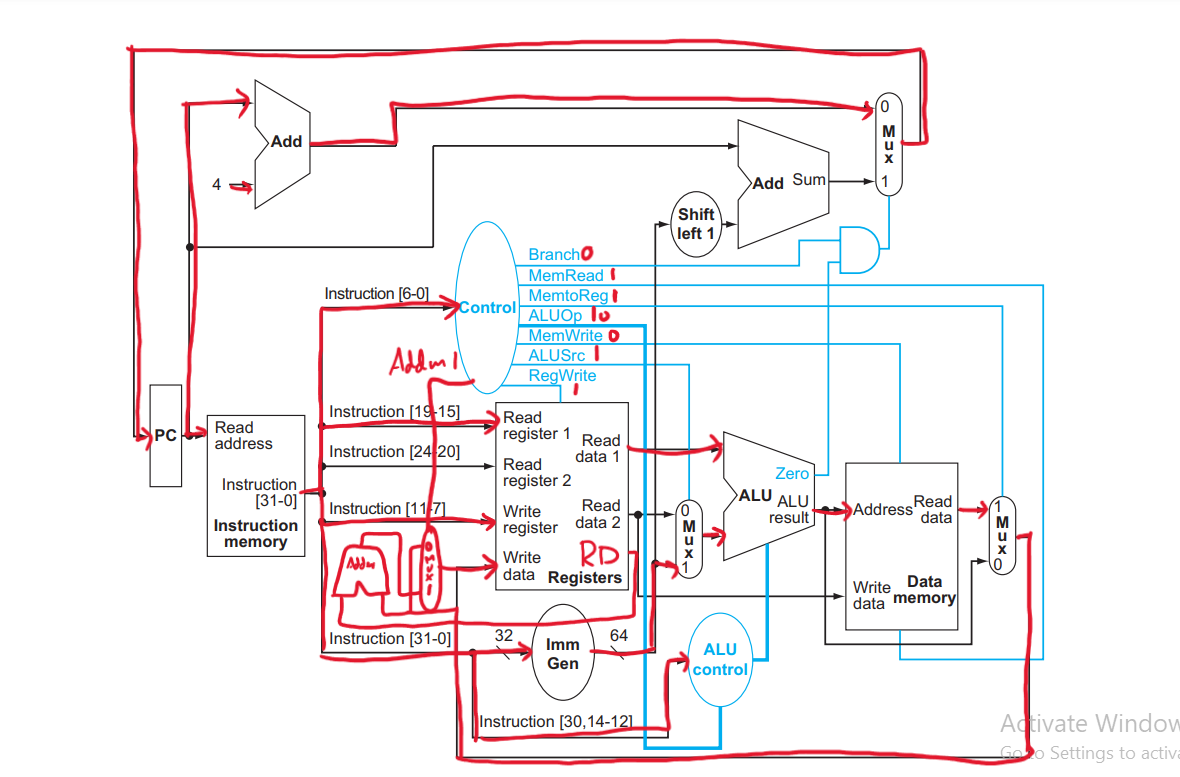
\includegraphics[scale = 0.5]{Q7_b_addtomem.png}
                \end{figure}
                
                \subpart It would increase the latency as the new instruction requires another signal ``Addm'' and additional hardware; Mux and Adder for the writeback.
                \subpart No new pipeline stages would be needed, but ``Addm'' signal would be needed till the MEM/WB pipeline after which in the writeback stage we will place the adder and Mux. As shown: 
                \begin{figure}[H]
                    \centering
                    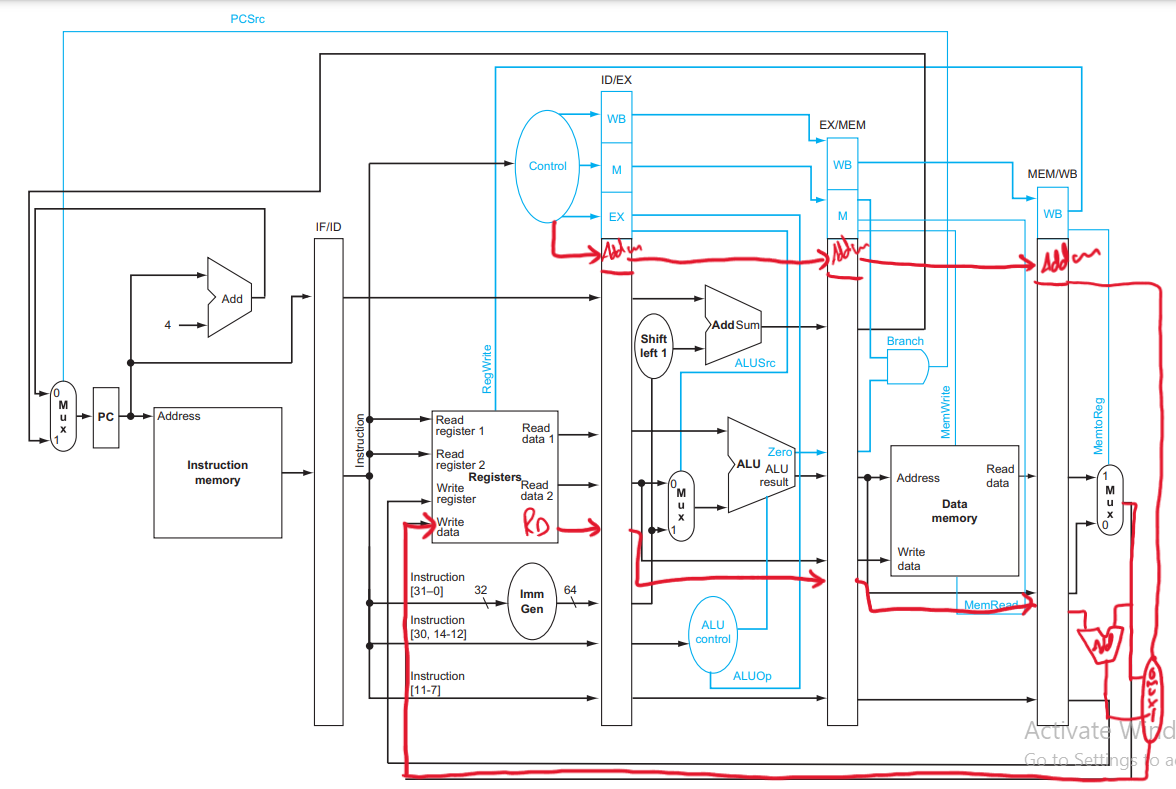
\includegraphics[scale = 0.5]{Q7_d_addtomem.png}
                \end{figure}
                \subpart There won't be any new data hazards but the same as before.
                \subpart RISC-V architecture is the simplest architecture. Adding this instruction would increase the complexity significantly, hence it was not added to the RISC-V architecture. Further, the same operation can be performed using an \texttt{ld} and an \texttt{add} instruction.
            \end{subparts}
            \newpage
            \part \underline{\texttt{Branch Equal to Memory}}
            
            \texttt{beqm rs1, offset(rs2), rs3} \hspace*{5mm} // if(Reg[rs1] == Mem[Offset + Reg[rs2]]) \\ 
             \hspace*{54mm} // \hspace*{10mm} PC = PC + Reg[rs3]
            \begin{subparts}
                \renewcommand{\thesubpart}{\alph{subpart}}
                \subpart There is no existing RISC-V instruction format that is suitable to encode this instruction as this branch instruction involves a memory access operand in the instruction. So we will have to define a new instruction such as ``BM-Type'' which denotes a branch instruction with memory access. The instruction format can then be 7-bit Opcode [custom], 5-bit RS1, 5-bit RS2, 5-bit RS3, 3-bit funct3 value [custom], and 7-bit immediate value.
                \subpart There is no WriteData or writeback, however, we need to access Memory along with offset on RS2, and then we need to perform ALU operation (a - b) to check for 0 value. If zero, then we need to increment PC value with RS3 value. RS3 is an input to Register File, and output is ReadData3 which is sent as an increment to the PC value counter. The datapath becomes:
                \subpart The latency would undoubtedly increase as now we have to assume branch is taken, then access the memory, then again access the ALU Stage to calculate branch, and in case the branch is true, then send a signal such that PC value is incremented by the value of RS3. So it would require more clock cycles or more time to execute, so latency increases.
                \subpart We would have to increase the number of pipeline stages to accomodate for the increase in hardware and increased clock cycles to allow the execution of instructions - an additional ALU might be considered.
                \subpart There won't be any new types of data hazards.
                \subpart RISC-V architecture is the simplest architecture. Adding this instruction would increase the complexity of the design significantly, as we need more signals, more hardware, and more pipeline stages. Hence it was not added to the RISC-V architecture.
            \end{subparts}
            \newpage
            \part \underline{\texttt{Store Word and Increment}}
            
            \texttt{swinc rs2, offset(rs1)} \hspace*{5mm} // Mem[Reg[rs1] + offset] = Reg[rs2], \\ \hspace*{47mm} // Reg[rs1] = Reg[rs1] + 4
            \begin{subparts}
                \renewcommand{\thesubpart}{\alph{subpart}}
                \subpart There is no existing RISC-V instruction format that can access the memory to store a value and also increment the value in a register simultaneously, however, we can use and modify the existing S-Type instruction format. The instruction format can then be 7-bit Opcode [custom], 5-bit Immediate, 3-bit Funct3 [custom], 5-bit RS1, 5-bit RS2, 7-bit Immediate.
                \subpart We would have a MemWrite where the write data is the value of RS2, and at the same time we would increment the value of RS1 by 4 using an adder, and a MUX controlled by a ``swinc'' signal as below:
                \begin{figure}[H]
                    \centering
                    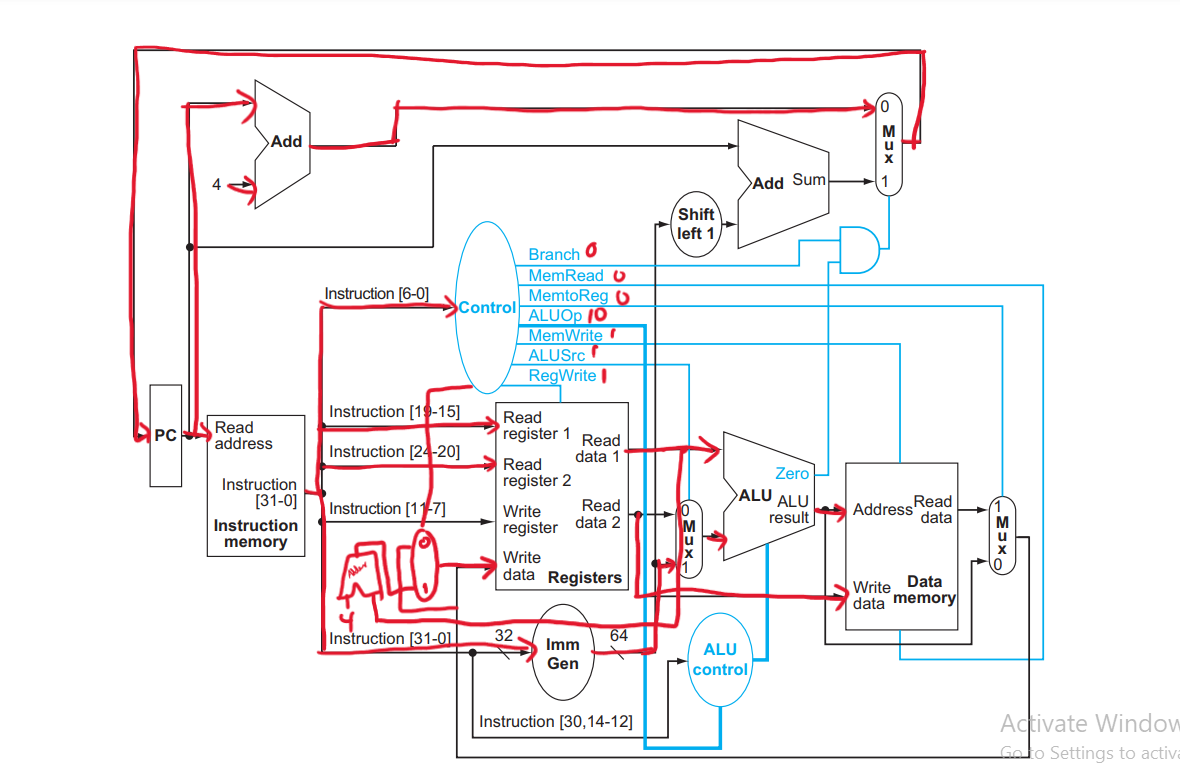
\includegraphics[scale = 0.5]{Q7_b_swinc.png}
                \end{figure}

                \subpart The latency would increase as we would now have to assert signals for accessing memory and incrementing the value of the register through additional hardware which would definitely take more time.
                \subpart There is no need for increasing pipeline stages, however, there will be more signals and hardware as shown:
                \begin{figure}[H]
                    \centering
                    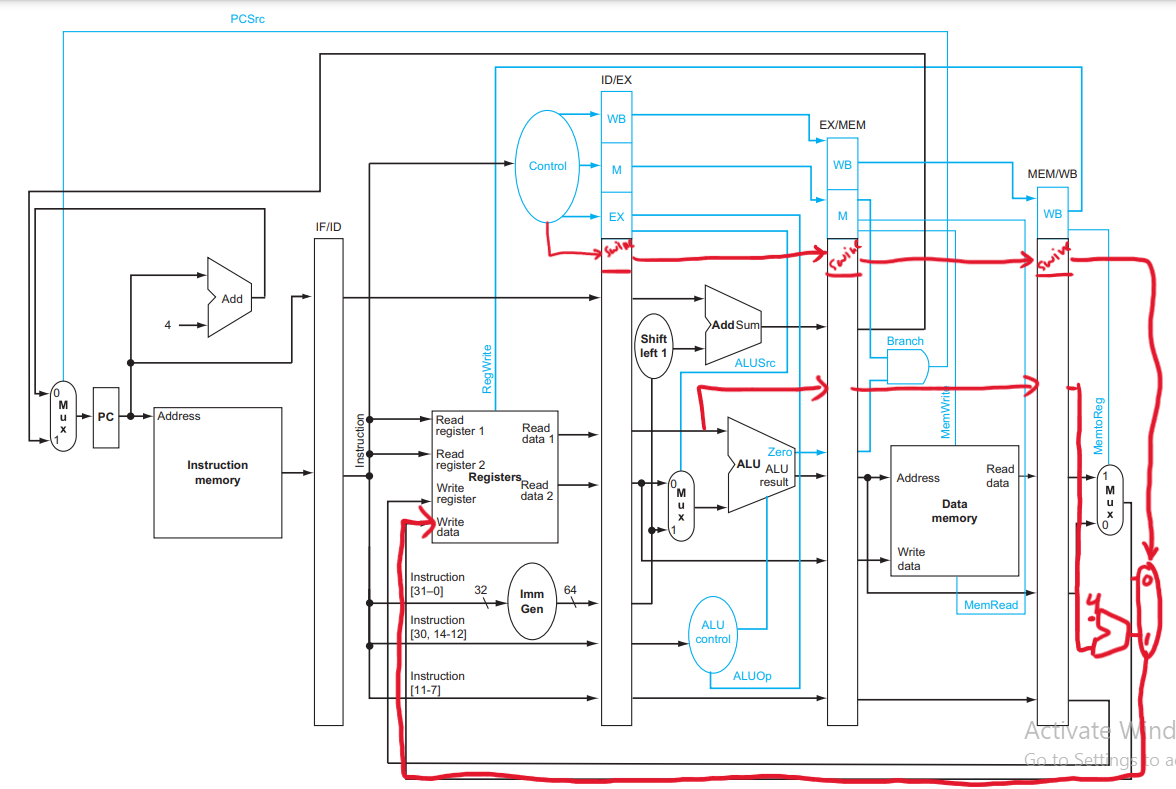
\includegraphics[scale = 0.5]{Q7_d_swinc.png}
                \end{figure}

                \subpart There are not going to be any new data hazards, however, there can be the control hazard which might not be mitigated by forwarding in each case and would have to stall.
                \subpart RISC-V architecture is the simplest architecture. Adding this instruction would increase the complexity of the design, hence it was not added to the RISC-V architecture. 
            \end{subparts}
        \end{parts}
    \end{solution}
    \pagebreak
    \question[5]
    \begin{center}
        \textbf{Question 8: Structural Hazard Analysis}
    \end{center}

    Consider the fragmant of the RISC-V assembly below:

    \begin{tabular}{l c l c}
        \texttt{ld} & \texttt{x31,} & \texttt{32(x10)} & \\ 
        \texttt{sd} & \texttt{x11,} & \texttt{8(x10)} & \\
        \texttt{sub} & \texttt{x12,} & \texttt{x14,} & \texttt{x13} \\ 
        \texttt{add} & \texttt{x15,} & \texttt{x12,} & \texttt{x13} \\ 
        \texttt{beq} & \texttt{x24,} & \texttt{x0,} & \texttt{label} \\ 
        \texttt{add} & \texttt{x31,} & \texttt{x31,} & \texttt{x14}
    \end{tabular}

    Suppose we modify the pipeline so that it has only one memory (that handles both instructions and data). In this case, there will be a structural hazard every time a program needs to fetch an instruction during the same cycle in which another instruction accesses data. 

    \begin{parts}
        \renewcommand{\thepartno}{\roman{partno}}
        \part Draw a pipeline diagram to show where the code above will stall. 
        \begin{solution}
            Stall has been highlighted with yellow in the figure below.
            \begin{figure}[H]
                \centering
                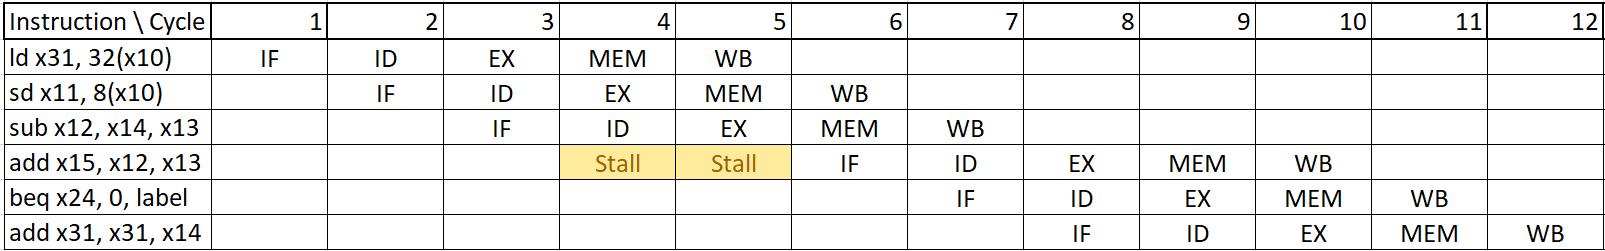
\includegraphics[scale = 0.385]{q8_ans_i.png}
            \end{figure}
        \end{solution}
        \part In general, is it possible to reduce the number of stalls/NOPs resulting from this structural hazard by reordering code?
        \begin{solution}
            Reordering can sometimes help, however, for this structural hazard, reordering the code will not help as every instruction must be fetched; hence we will encounter a stall every time data has to be accessed. 
        \end{solution}
        \part Must this structural hazard be handled in hardware? We have seen that data hazards can be eliminated by adding NOPs to the code. Can you do the same with this sturctural hazard? If so, explain how. If not, explain why not.
        \begin{solution}
            NOPs will also have to be fetched from the Instruction Memory, so again in the fetching stage, there will be a stall. So adding NOPs will not resolve the structural hazard.
        \end{solution}
        \part Approximately how many stalls would you expect this structural hazard to generate in a typical program? Use this instruction mix from Question 2.
        \begin{solution}
            Since every data access would cause a stall, then stall would occur each time Data Memory is accessed; load and store instructions. 

            Then we would expect stall on 20\% + 25\% = 45\% of the instructions using the instruction mix from Question 2.
        \end{solution}
    \end{parts}
% \pagebreak
    \question[5]
    \begin{center}
        \textbf{Question 9: Forwarding/Hazard-Detection Units Analysis [5 marks]}
    \end{center}

    Problems in this exercise refer to the following sequence of instructions, and assume that it is executed on a five-stage pipelined datapath.

    \begin{tabular}{l c l l}
        \texttt{and} & \texttt{x16,} & \texttt{x10,} & \texttt{x9} \\ 
        \texttt{ld} & \texttt{x29,} & \texttt{4(x16)} & \\
        \texttt{ld} & \texttt{x10,} & \texttt{0(x2)} & \\ 
        \texttt{sub} & \texttt{x29,} & \texttt{x29,} & \texttt{x15} \\ 
        \texttt{sd} & \texttt{x29,} & \texttt{0(x16)}
    \end{tabular}

    \begin{parts}
        \renewcommand{\thepartno}{\roman{partno}}
        \part If there is no forwarding or hazard detection, insert NOPs to ensure correct execution.
        \begin{solution}
            There will be two stalls after \texttt{and} instruction, as the next instruction uses the destination register of \texttt{and}. There will be a stall after ld instruction, and two stalls after sub instruction. Then we have to insert NOPs at these occurances. 
            \begin{tabular}{l c l l}
                \texttt{and} & \texttt{x16,} & \texttt{x10,} & \texttt{x9} \\ 
                \texttt{NOP} & & & \\
                \texttt{NOP} & & & \\
                \texttt{ld} & \texttt{x29,} & \texttt{4(x16)} & \\
                \texttt{ld} & \texttt{x10,} & \texttt{0(x2)} & \\ 
                \texttt{NOP} & & & \\
                \texttt{sub} & \texttt{x29,} & \texttt{x29,} & \texttt{x15} \\ 
                \texttt{NOP} & & & \\
                \texttt{NOP} & & & \\
                \texttt{sd} & \texttt{x29,} & \texttt{0(x16)}
            \end{tabular}

        \end{solution}
        \part Now, change and/or rearrange the code to minimize the number of NOPs needed. You can assume register x17 can be used to hold temporary values in your modified code.
        \begin{solution}
            NOPs won't be reduced by reordering the code in this case.
        \end{solution}
        \part If the processor has forwarding, but we forgot to implement the hazard detection unit, what happens when the original code executes?
        \begin{solution}
            The code will still execute without any complications as hazard detection is needed in case of a load instruction such that it uses the result of the previous load instruction which is not happening in the given sequence of instructions.
        \end{solution}
        \pagebreak
        \part If the processor has forwarding, for the first seven cyces during the execution of this code, specify which signals are asserted in each cycle by hazard detection and forwarding units in Figure 4.59 of the book.
        \begin{solution}
            \begin{figure}[H]
                \centering
                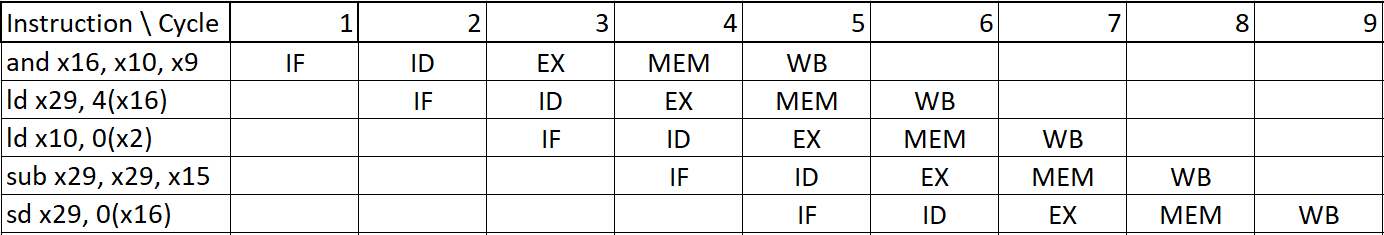
\includegraphics[scale = 0.445]{q9_ans_iv.png}
            \end{figure}
            There are no stalls for the given sequence of instructions, and there would be no signals asserted by the hazard detection unit.

            No execution for the first two cycles, so no forwarding. \\ 
            (3) First execution, ForwardA = 00, ForwardB = 00 \\ 
            (4) Need for forwarding ALU Result to ld; ForwardA = 10, ForwardB = 00\\ 
            (5) No forwading; ForwardA = 00, ForwardB = 00 \\ 
            (6) Need for forwarding result of ld to sub; ForwardA = 00, ForwardB = 01 \\ 
            (7) Need for forwarding result of sub to sd; Forward A = 10, ForwardB = 00.
            
            \vspace*{2mm}
            *[The above ForwardA and ForwardB values are in binary as from the book]
        \end{solution}
        \part If there is no forwarding, what new input and output signals do we need for the hazard detection unit in Figure 4.59? Using this instruction seqeunce as an example, explain why each signal is needed.
        \begin{solution}
            The hazard detection unit would additionally need to check if the result of the previous instruction is being used by the current/next instruction, in which case it would need to forward the result. So the hazard detection unit would need the rd values from the MEM/WB register. If the new instruction in the ID needs the result of the previous instruction, then the current instruction in the ID would be stalled. So the rd values of both the registers would have to be compared. The hazard unit would already have the destination register from the EX/MEM register, so only the value from MEM/WB has to be sent to the hazard detection unit. \\ 
            So no additional outputs will be needed, and the pipeline can be stalled with the existing signals by just reconnecting them. 

            Using this instruction seqeunce as an example, the value of rd from EX/MEM is needed to detect the data hazard between \texttt{and} and the \texttt{ld} instruction. The value of rd from MEM/WB is needed to detect the data hazard between the first \texttt{ld} instruction and \texttt{sub} instruction.  
        \end{solution}
        \pagebreak
        \part For the new hazard detection unit form (v), specify which output signals it asserts in each of the first five-cycles during the execution of this code.
        \begin{solution}
            \begin{figure}[H]
                \centering
                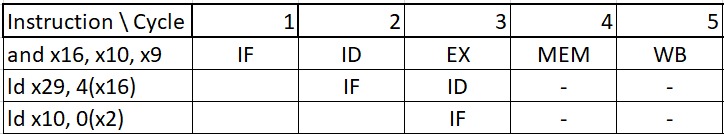
\includegraphics[scale = 0.85]{q9_ans_vi.png}
            \end{figure}

            In the first three cycles, PCWrite = 1, IF/ID Write = 1, and control mux = 0 as there is no data hazard, so no stall or forwarding required and things operate as normal. 

            (4) PCWrite = 0, IF/ID Write = 0, control mux = 1 as there is a hazard now so we need to stall the instruction. \\ 
            (5) PCWrite = 0, IF/ID Write = 0, control mux = 1 due to hazard and need for stall.
        \end{solution}
    \end{parts}

    \question[5]
    \begin{center}
        \textbf{Question 10: Forwarding Trade-Offs [5 marks]}
    \end{center}

    Consider the pipelined RISC-V version with 5 stages discussed in class that does not handle data hazards (i.e., the programmer is responsible for addressing data hazards by inserting NOP instructions where necessary). Suppose that (after optimization) a typical n-instruction program requires an additional 0.3*n NOP instructions to correctly handle data hazards.

    \begin{parts}
        \renewcommand{\thepartno}{\roman{partno}}
        \part Suppose that the cycle time of this pipeline without forwarding is 200ps. Suppose also that adding forwarding hardware will reduce the number of NOPs from 0.3*n to 0.06*n, but increase the cycle time to 250ps. What is the speedup of this new pipeline compared to the one without forwarding?
        \begin{solution}
            Pipeline without forwarding takes $ 1.3 * n * 200ps = 260n$. \\ 
            Pipeline with forwarding takes $ 1.06 * n * 250ps = 265n $ \\ 
            Speedup = $ \displaystyle\frac{260}{265} = 0.98 $ 
        \end{solution}
        \part Different programs will require different amounts of NOPs. How many NOPs (as a percentage of code instructions) can remain in the typical program before that program runs slower on the pipeline with forwarding?
        \begin{solution}
            Pipeline with forwarding must be faster than the pipeline without the forwarding. Then $ 250 * (1 + s) * n < 200 * 1.3 * n $ where $s$ is the number of stalls. 

            Then $ 1 + s < 1.04 \implies s < 0.04 $.

            So $s$ must be less than 4\%. 
        \end{solution}
        \part Repeat (ii); however, this time let x represent the number of NOP instructions relative to n. (In (ii), x was equal to 0.3) Your answer will be with respect to x.
        \begin{solution}
            Now we have $x$ relative to our answer in part (ii) where $x$ is the number of NOPs relative to n. Then $ 250 * (1 + s)*n < 200*(1+x)*n $.

            Then $ 1 + s < \displaystyle\frac{4(1+x)}{5} $ \\ $ \implies s < \displaystyle\frac{4 + 4x - 5}{5} \implies s < \displaystyle\frac{4x - 1}{5} $
        \end{solution}
        \part Can a program with only .075*n NOPs (in the no-forwarding case) possibly run faster on the pipeline with forwarding? Explain why or why not.
        \begin{solution}
            We have $ 0.075*n $ NOPs. With forwarding, the program takes $ 250ps $ while without forwarding, the program takes $ 200 * 1.075 = 215ps $. Hence it will not be able to run faster. 
        \end{solution}
        \part At minimum, how many NOPs (as a percentage of code instructions) must a program have before it can possibly run faster on the pipeline with forwarding?
        \begin{solution}
            We need the program to run faster on the pipeline with forwarding, therefore speedup must be positive. 

            Then $ \displaystyle\frac{4x - 1}{5} > 0 \implies x > 0.25 $. Then at minimum, the program must have at least 0.25 NOPs to run faster on the pipeline with forwarding.
        \end{solution}
    \end{parts}
    \pagebreak
    \question[5]
    \begin{center}
        \textbf{Question 11: Forwarding Logic Design Trade-Offs [5 marks]}
    \end{center}

    This exercise is intended to help you understand the cost/complexity/ performance trade-offs of forwarding in a pipelined processor. Problems in this exercise refer to pipelined datapaths from Figure 4.53 of the book. These problems assume that, of all the instructions executed in a processor, the following fraction of these instructions has a particular type of read-after-write (RAW) data dependence.

    \begin{figure}[ht]
        \centering
        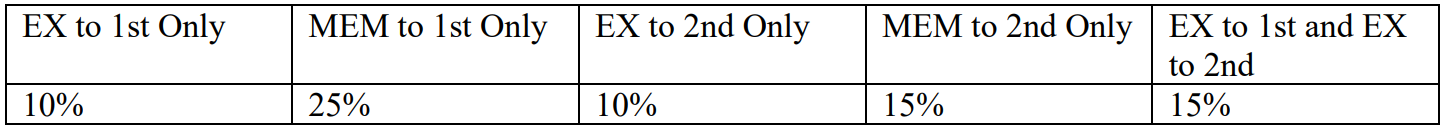
\includegraphics[scale = 0.45]{q11_figi.png}
    \end{figure}

    The type of RAW data dependence is identified by the stage that produces the result (EX or MEM) and the next instruction that consumes the result (1st instruction that follows the one that produces the result, 2nd instruction that follows, or both). We assume that the register write is done in the first half of the clock cycle and that register reads are done in the second half of the cycle, so “EX to 3rd” and “MEM to 3rd” dependences are not counted because they cannot result in data hazards. We also assume that branches are resolved in the EX stage (as opposed to the ID stage), and that the CPI of the processor is 1 if there are no data hazards.

    Assume the following latencies for individual pipeline stages. For the EX stage, latencies are given seprately for a processor without forwarding and for a processor with different kinds of forwarding.

    \begin{figure}[ht]
        \centering
        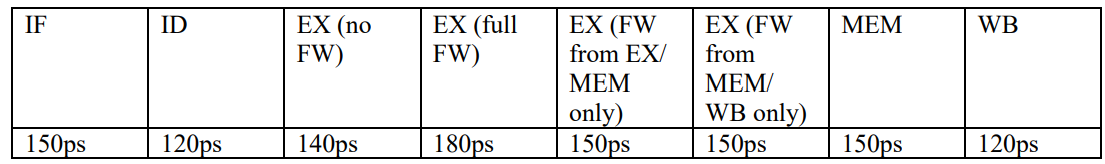
\includegraphics[scale = 0.63]{q11_figii.png}
    \end{figure}

    \begin{parts}
        \renewcommand{\thepartno}{\roman{partno}}
        \part For each RAW dependancy listed above, give a sequence of at least three assembly statements that exhibits that dependancy.
        \begin{solution}

            (1) \textbf{EX to 1st Only:} \\ 
            \hspace*{3mm} \begin{tabular}{l l l l}
                \texttt{add} & \texttt{x5,} & \texttt{x6,} & \texttt{x7} \\ 
                \texttt{add} & \texttt{x8,} & \texttt{x5,} & \texttt{x9} \\ 
                \texttt{add} & \texttt{x10,} & \texttt{x11,} & \texttt{x12}
            \end{tabular}

            (2) \textbf{MEM to 1st Only:} \\ 
            \hspace*{3mm} \begin{tabular}{l l l l}
                \texttt{ld} & \texttt{x10,} & \texttt{0(x12)} & \\ 
                \texttt{add} & \texttt{x11,} & \texttt{x10,} & \texttt{x13} \\ 
                \texttt{add} & \texttt{x5,} & \texttt{x6,} & \texttt{x7}
            \end{tabular}

            (3) \textbf{EX to 2nd Only:} \\ 
            \hspace*{3mm} \begin{tabular}{l l l l}
                \texttt{add} & \texttt{x5,} & \texttt{x6,} & \texttt{x7} \\ 
                \texttt{add} & \texttt{x10,} & \texttt{x11,} & \texttt{x12} \\ 
                \texttt{add} & \texttt{x8,} & \texttt{x5,} & \texttt{x9}
            \end{tabular}

            (4) \textbf{MEM to 2nd Only:} \\ 
            \hspace*{3mm} \begin{tabular}{l l l l}
                \texttt{ld} & \texttt{x10,} & \texttt{0(x12)} & \\ 
                \texttt{add} & \texttt{x5,} & \texttt{x6,} & \texttt{x7} \\ 
                \texttt{add} & \texttt{x11,} & \texttt{x10,} & \texttt{x13} 
            \end{tabular}

            (5) \textbf{EX to 1st and EX to 2nd:} \\ 
            \hspace*{3mm} \begin{tabular}{l l l l}
                \texttt{add} & \texttt{x5,} & \texttt{x6,} & \texttt{x7} \\ 
                \texttt{add} & \texttt{x8,} & \texttt{x5,} & \texttt{x9} \\ 
                \texttt{add} & \texttt{x10,} & \texttt{x5,} & \texttt{x11}
            \end{tabular}
        \end{solution}
        \part For each RAW dependancy above, how many NOPs would need to be inserted to allow your code from (i) to run correctly on a pipeline with no forwarding or hazard detection? Show where the NOPs could be inserted. 
        \begin{solution}
            
            (1) \textbf{EX to 1st Only:} 2 NOPs \\ 
            \hspace*{3mm} \begin{tabular}{l l l l}
                \texttt{add} & \texttt{x5,} & \texttt{x6,} & \texttt{x7} \\ 
                \texttt{NOP} \\ \texttt{NOP} \\
                \texttt{add} & \texttt{x8,} & \texttt{x5,} & \texttt{x9} \\ 
                \texttt{add} & \texttt{x10,} & \texttt{x11,} & \texttt{x12}
            \end{tabular}

            (2) \textbf{MEM to 1st Only:} 2 NOPs\\ 
            \hspace*{3mm} \begin{tabular}{l l l l}
                \texttt{ld} & \texttt{x10,} & \texttt{0(x12)} & \\ 
                \texttt{NOP} \\ \texttt{NOP} \\ 
                \texttt{add} & \texttt{x11,} & \texttt{x10,} & \texttt{x13} \\ 
                \texttt{add} & \texttt{x5,} & \texttt{x6,} & \texttt{x7}
            \end{tabular}

            (3) \textbf{EX to 2nd Only:} 1 NOP\\ 
            \hspace*{3mm} \begin{tabular}{l l l l}
                \texttt{add} & \texttt{x5,} & \texttt{x6,} & \texttt{x7} \\ 
                \texttt{add} & \texttt{x10,} & \texttt{x11,} & \texttt{x12} \\ \texttt{NOP} \\
                \texttt{add} & \texttt{x8,} & \texttt{x5,} & \texttt{x9}
            \end{tabular}

            (4) \textbf{MEM to 2nd Only:} 1 NOP \\ 
            \hspace*{3mm} \begin{tabular}{l l l l}
                \texttt{ld} & \texttt{x10,} & \texttt{0(x12)} & \\ 
                \texttt{add} & \texttt{x5,} & \texttt{x6,} & \texttt{x7} \\ \texttt{NOP} \\ 
                \texttt{add} & \texttt{x11,} & \texttt{x10,} & \texttt{x13} 
            \end{tabular}

            (5) \textbf{EX to 1st and EX to 2nd:} 2 NOPS \\ 
            \hspace*{3mm} \begin{tabular}{l l l l}
                \texttt{add} & \texttt{x5,} & \texttt{x6,} & \texttt{x7} \\ 
                \texttt{NOP} \\ \texttt{NOP} \\ 
                \texttt{add} & \texttt{x8,} & \texttt{x5,} & \texttt{x9} \\ 
                \texttt{add} & \texttt{x10,} & \texttt{x5,} & \texttt{x11}
            \end{tabular}
        \end{solution}
        \pagebreak
        \part Analyzing each instruction independently will over-count the number of NOPs needed to run a
        program on a pipeline with no forwarding or hazard detection. Write a sequence of three assembly instructions so that, when you consider each instruction in the sequence independently, the sum of the stalls is larger than the number of stalls the sequence actually needs to avoid data hazards.
        \begin{solution}
            A possible code can be considered: \\ 
            \begin{tabular}{l l l l l}
                \texttt{ld} & \texttt{x10,} & \texttt{0(x12)} & & \# MEM to 2nd: 1 NOP \\ 
                \texttt{add} & \texttt{x5,} & \texttt{x6,} & \texttt{x7} & \# EX to 1st: 2 NOPs \\ 
                \texttt{add} & \texttt{x11,} & \texttt{x10,} & \texttt{x5} \\ 
                \texttt{add} & \texttt{x28,} & \texttt{x29,} & \texttt{x30} 
            \end{tabular}

            Individually if the code is analysed, then we would have 3 NOPs, 1 from the first ld instruction and 2 from the second add instruction. However, when the code will be executed, there will only be 2 NOPs, or 2 stalls occuring only after the second add instruction, as there is overlap between the NOPs resulting from the first ld instruction, and the second add instruction, hence the sum of NOPs from the code is less than the sum of NOPs obtained after analysing each instruction individually. 

            Like so: 

            \begin{tabular}{l l l l l}
                \texttt{ld} & \texttt{x10,} & \texttt{0(x12)} & & \# MEM to 2nd: 1 NOP \\ 
                \texttt{add} & \texttt{x5,} & \texttt{x6,} & \texttt{x7} & \# EX to 1st: 2 NOPs \\ 
                \texttt{NOP} \\ \texttt{NOP} \\ 
                \texttt{add} & \texttt{x11,} & \texttt{x10,} & \texttt{x5} \\ 
                \texttt{add} & \texttt{x28,} & \texttt{x29,} & \texttt{x30} 
            \end{tabular}

        \end{solution}
        \part Assuming no other hazards, what is the CPI for the program described by the table above when run on a pipeline with no forwarding? What percent of cycles are stalls? (For simplicity, assume that all necessary cases  are listed above and can be treated independently.)
        \begin{solution}
            We can take an average of the codes used in (ii) to get an estimate of stalls per instruction. 

            Average = $ 2\times10\% + 2\times25\% + 1\times10\% + 1\times15\% + 2\times15\% = 1.25 $ stalls per instruction on average for a CPI of 2.25. Then on average, there are $ \displaystyle\frac{1.25}{2.25} = 0.556 $ cycles or 55.6\% stalls.
        \end{solution}
        \part What is the CPI if we use full forwarding (forward all results that can be forwarded)? What percent of cycles are stalls?
        \begin{solution}
            The only dependancy that can not be handled by forwarding is the MEM to 1st dependancy - forwarding from MEM stage to the next instruction. Then 25\% of instructions will generate 1 stall. Then there are $ \displaystyle\frac{0.25}{1.25} = 0.2 $ cycles or 20\% stalls.
        \end{solution}
        \pagebreak
        \part Let us assume that we cannot afford to have three-input multiplexors that are needed for full forwarding. We have to decide if it is better to forward only from the EX/MEM pipeline register (next-cycle forwarding) or only from the MEM/WB pipeline register (two-cycle forwarding). What is the CPI for each option?
        \begin{solution}
            
            (1) \textbf{From EX/MEM:} \\ 
            \hspace*{5mm} Stalls from forwarding from EX/MEM are 0 in EX to 1st, 2 in MEM to 1st, \\ \hspace*{5mm} 1 in EX to 2nd, 1 in MEM to 2nd, and 1 in EX to 1st and 2nd. Then we get an \hspace*{5mm} average of $ 0\times10\% + 2\times25\% + 1\times10\% + 1\times15\% + 1\times15\% = 0.9 $ stalls per \hspace*{5mm} instruction. \textbf{CPI = 1.9.}

            (2) \textbf{From MEM/WB:} \\ 
            \hspace*{5mm} Stalls are 1 in Ex to 1st, 1 in MEM to 1st, 0 in EX to 2nd, 0 in MEM to 2nd, \\ \hspace*{5mm} 1 in EX to 1st and 2nd. Then on average $ 1\times10\% + 1\times25\% + 0\times10\% + \\ \hspace*{6mm} 0\times15\% + 1\times15\% = 0.5 $ stalls per instruction. \textbf{CPI = 1.5.}
        \end{solution}
        \part For the given hazard probabilities and pipeline stage latencies, what is the speedup achieved by each type of forwarding (EX/MEM, MEM/WB, for full) as compared to a pipeline that has no forwarding?
        \begin{solution}
            The following table shows the necessary information required to calculate the relative speedup of each type of forwarding as compared to a pipeline without forwarding.

            \begin{figure}[H]
                \centering
                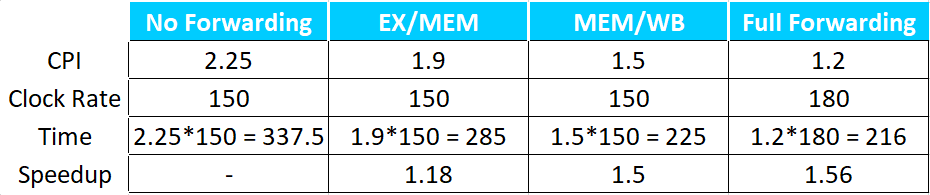
\includegraphics[scale = 0.65]{q11_ans_vii.png}    
            \end{figure}
        \end{solution}
        \part What would be the additional speedup (relative to the fastest processor from (vii)) be if we added  ``time-travel'' forwarding that eliminates all data hazards? Assume that the yet-to-be-invented time-travel circuitry adds 100ps to the latency of the full-forwarding EX stage.
        \begin{solution}

            \begin{tabular}{l c c c }
                MEM/WB: & CPI = 1.5, & Clock Rate = 150, & Time = 225\\ 
                Time Travel: & CPI = 1.00, & Clock Rate = 280, & Time = 280.0 
            \end{tabular}

            Speedup by time travel = $ \displaystyle\frac{225}{280} = 0.80 $

            The additional speedup relative to the fastest processor from vii is of 0.80 which means that time-travel would slow the processor further if it adds 100ps to the latency of the full forwarding.
        \end{solution}
        \part The table of hazard types has seperate entries for ``EX to 1st'' and ``EX to 1st and EX to 2nd''. Why is there no entry for ``MEM to 1st and MEM to 2nd''?
        \begin{solution}
            From part (vi), we can see that in the EX/MEM stage, there is no stall from EX to 1st, but there is one stall from EX to 1st and 2nd. However, MEM to 1st and MEM to 1st and 2nd both will have the same number of stalls - all MEM to 1st will cause a stall due to which the second instruction's ID overlaps with the original instruction's WB. Hence there is no entry for MEM to 1st and MEM to 2nd. 
        \end{solution}
    \end{parts}

\end{questions}
\end{sloppypar}
\end{document}